\chapter{Implementation}

\section{Introduction}
This chapter details the implementation phase of our project, which follows an agile methodology with four sprints. Each sprint focuses on delivering specific features and functionality according to the project backlog.

\section{Sprint 1: Authentication and User Management}
\subsection{Overview}
The first sprint focuses on establishing the core authentication system and user management functionality. This foundation is critical for all subsequent features as it defines user roles and access controls.

\subsection{User Types}
The system supports three distinct user types, each with different permissions and capabilities:
\begin{itemize}
    \item \textbf{Super Admin}: Has complete access to all system features and can manage admins and agents.
    \item \textbf{Admin}: Can manage agents and has access to administrative features within their assigned scope.
    \item \textbf{Agent}: Has limited access to the system based on their assigned responsibilities.
\end{itemize}

\subsection{Authentication System}
\subsubsection{Sign-up Process}
The sign-up process is illustrated in Figure \ref{fig:signup-diagram} below. The diagram shows the authentication flow for new users registering in the system.

\begin{figure}[ht!]
    \centering
    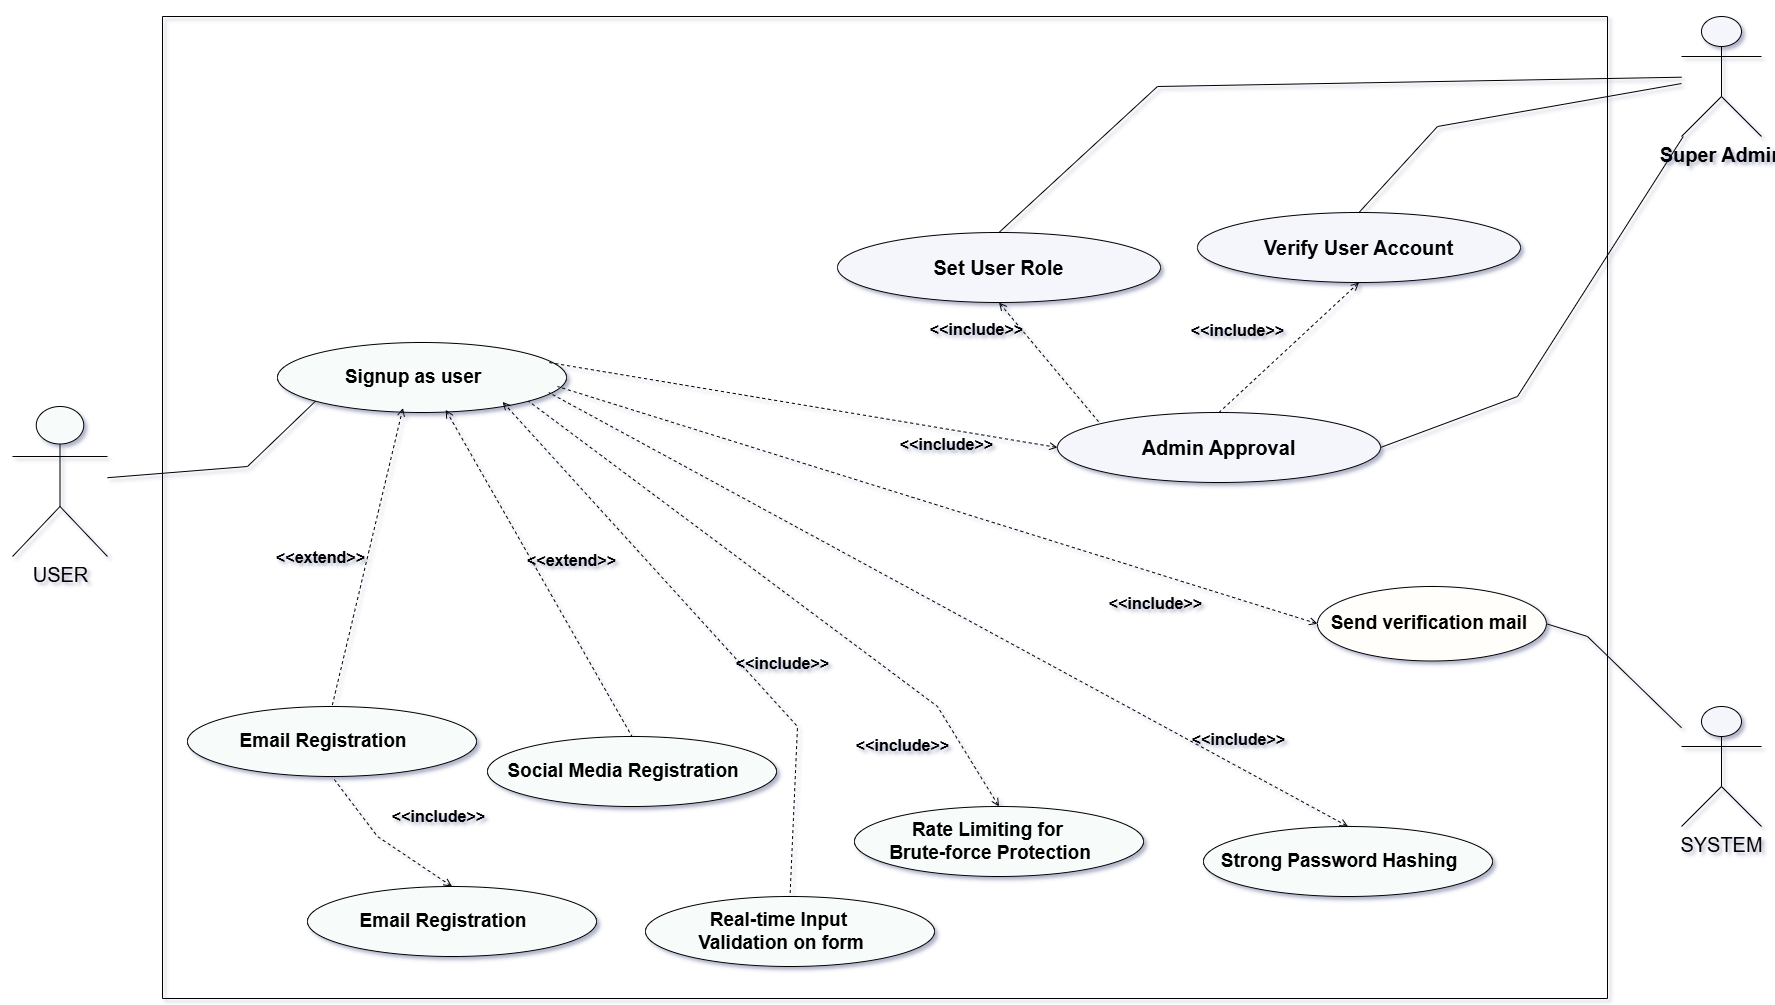
\includegraphics[width=1\textwidth]{images/diagram_de_case_d_utilisation_signup.png}
    \caption{Authentication Sign-up Use Case Diagram}
    \label{fig:signup-diagram}
\end{figure}

% \vspace{1cm}
\newpage

The sign-up process includes user registration, role assignment, and account verification steps. During registration, users are categorized into one of the three user types: Super Admin, Admin, or Agent, with each type having different permissions and access levels within the system.

\subsection{Sprint 1 Deliverables}
The key deliverables for Sprint 1 include:

\subsubsection{Web Backoffice Authentication}
\begin{itemize}
    \item Admin dashboard login and authentication system
    \item Role-based access control for backoffice users (Super Admin, Admin, Agent)
    \item User management interface for creating and managing user accounts
    \item Permission management system for different user roles
    \item Security logs and audit trails for backoffice activities
    \item Session management and secure token handling
\end{itemize}
\subsubsection{Blockchain Foundation}
\begin{itemize}
    \item Blockchain architecture setup and configuration
    \item Smart contract development for property transactions
    \item Implementation of test transactions in blockchain test environment
    \item Integration of blockchain APIs with backend services
    \item Transaction validation and verification mechanisms
    \item Wallet creation and key management system
\end{itemize}

\subsubsection{AI Property Evaluation System}
\begin{itemize}
    \item AI model development for rent price prediction
    \item Property sale value estimation algorithm
    \item Data collection and preprocessing pipeline for real estate information
    \item Training environment setup for prediction models
    \item Integration of prediction APIs with property management system
    \item Evaluation dashboard for property value assessments
\end{itemize}

\subsubsection{DevOps Infrastructure}
\begin{itemize}
    \item CI/CD pipeline configuration on GitHub for backend services
    \item GCP Cloud Run integration for containerized deployment
    \item Automated testing and deployment workflow
    \item Initial Docker setup for application components:
        \begin{itemize}
            \item Frontend container configuration
            \item Mobile application build environment
            \item Web application container
            \item Backend API services container
            \item Nginx configuration for routing and load balancing
            \item AI services containerization
        \end{itemize}
    \item Monitoring and logging infrastructure setup
\end{itemize}

\subsubsection{Mobile Application}
\begin{itemize}
    \item Mobile authentication screens and functionality
    \item Biometric authentication integration
    \item Investment properties listing interface
    \item Property search and filtering functionality
    \item User profile management on mobile
    \item Push notification system for investment opportunities
\end{itemize}

% Additional sections for subsequent sprints will be added later 